\documentclass{article}

\usepackage{eso-pic,graphicx}
\usepackage[top=2cm, bottom=2cm, paperwidth=8in, paperheight=8in]{geometry}

\tracinglostchars=2
\usepackage[UTF8, fontset=none]{ctex} %Chinese

\setmainfont{URW Gothic L}[Scale=1.0]

\renewcommand{\abstractname}{Welcome to the world of Cosmoose!}
\usepackage{xcolor}


\usepackage[version=4]{mhchem} %chemical

\usepackage{verse}
\pagenumbering{gobble}
\setlength\parindent{0pt}

\usepackage{hyperref} %hyperlinks

\usepackage{graphicx}

\definecolor{darkcyan}{rgb}{0.07, 0.26, 0.26}
\definecolor{darksienna}{rgb}{0.24, 0.08, 0.08}

\newcommand{\bo}[1] {\textbf{#1}}
\newcommand{\bblu}[1] {\textbf{\textcolor{darkcyan}{#1}}}
\newcommand{\bbro}[1] {\textbf{\textcolor{darksienna}{#1}}}

\newcommand{\bckg}[1]{\AddToShipoutPictureBG*{\includegraphics[width=\paperwidth,height=\paperheight]{#1}}}

\urlstyle{same}

\begin{document}

%% title page
\bckg{img/bg}
\begin{center}
    
\includegraphics[height=.2\paperheight]{img/cclogo}

    
\includegraphics[height=.5\paperheight]{img/loading}
    %CC's road to Stardom: Guidebook

    \vspace{.5cm}
    {\Huge \bo{CC's Road to Stardom Guide}}
\end{center}

\clearpage

\poemtitle{Story}
\bckg{img/bg}

CC lives with the Cosmoose gang since they rescued him.
They are space pirates, on the run from the Earth government. Is all that really important?
Not that much, since it's his Birthday! Will his dream come true?

\begin{center}
    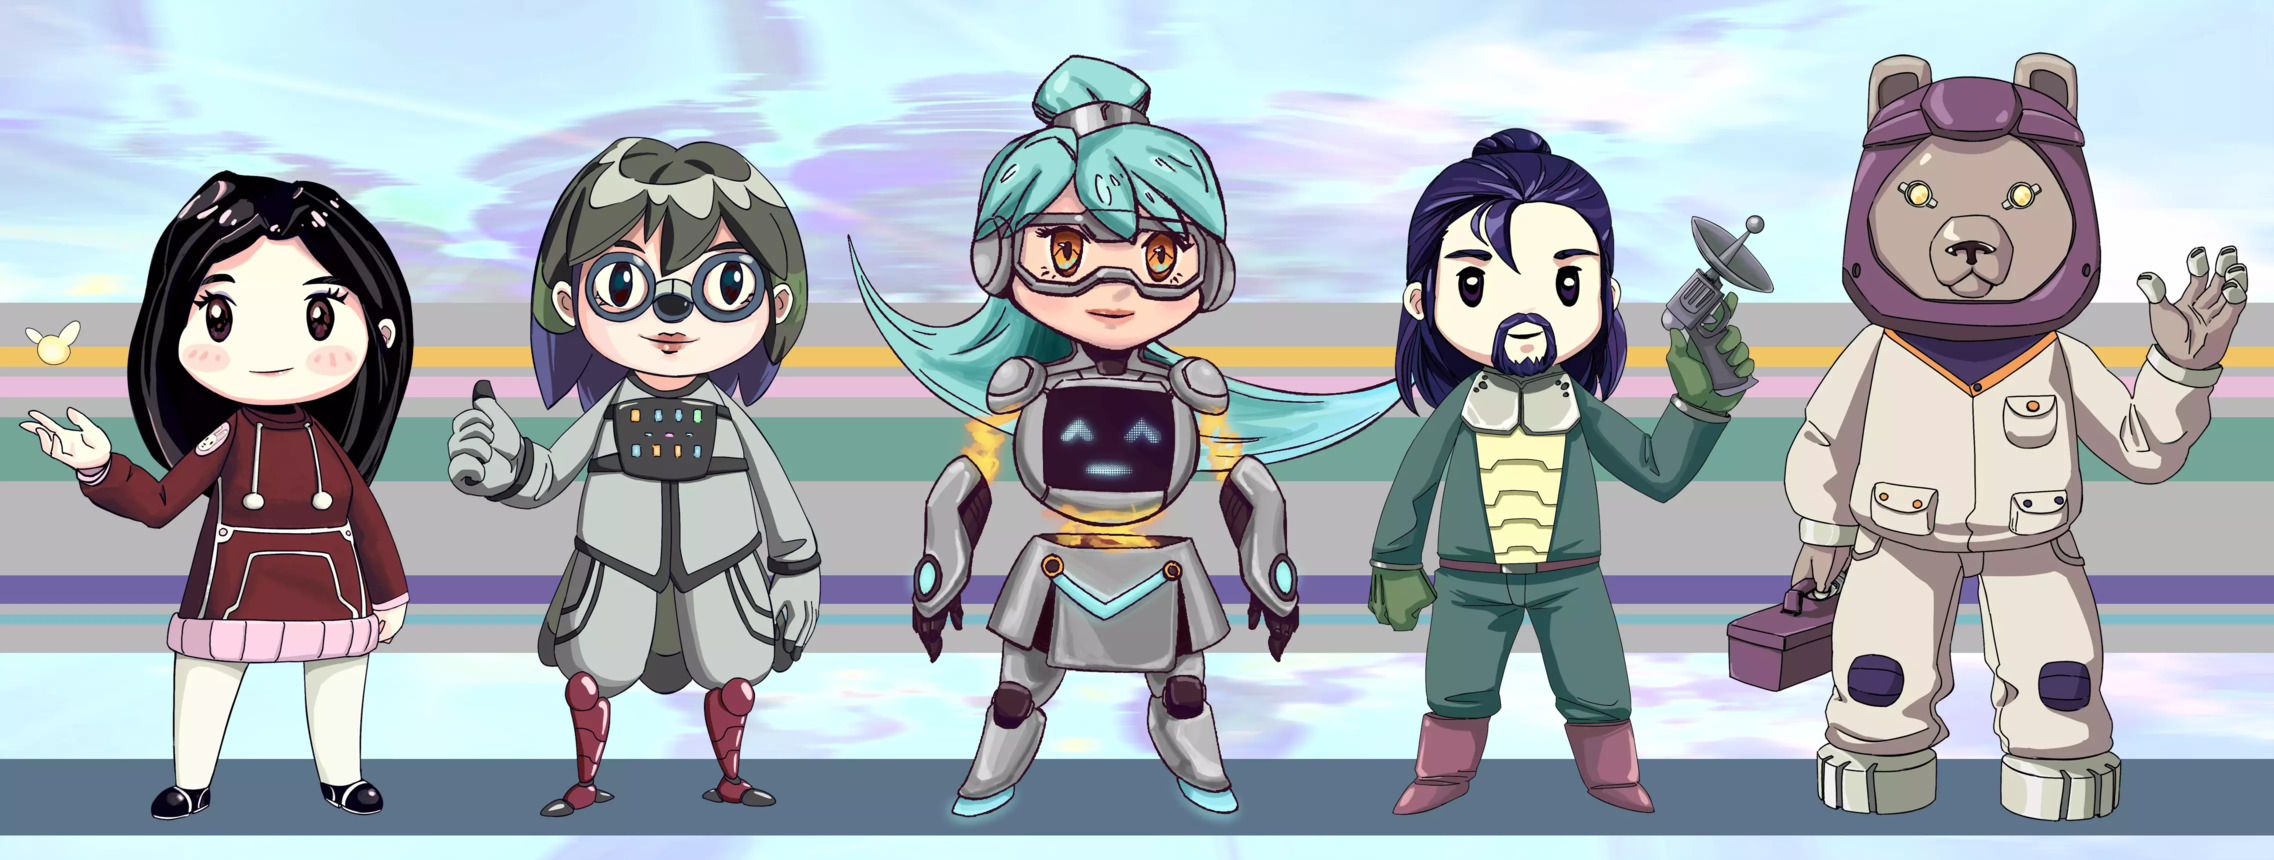
\includegraphics[height=.2\paperheight]{img/crew}
\end{center}

In this adventure, you are CC.
Here are all of your friends, from left to right:
\begin{itemize}
    \item Florrie, the nicest person on the ship! But she left for her programming certification...
    \item June, the inventor, who just gave you a mirror! What a good idea, we all need more beauty in our life!
    \item 7Cs, the ship AI, who's a robot who knows a lot about everything.
    \item Ru D., the captain, who you don't see too much as he's always gaming.
    \item Wool, who's probably nice, you're not sure, because you don't really understand what he says.
\end{itemize}

With their help, you will become the number 1 idol in the universe. Or so is the plan.

\clearpage
\poemtitle{Playing the game}
\bckg{img/bg}

This is a classical text adventure game.
To act, you need to input a \texttt{VERB} and a \texttt{SUBJECT}, or simply a \texttt{VERB}.
You'll need to \texttt{EXAMINE} your surroundings and the various objects you can find,
or \texttt{LOOK}; there are various synonyms accepted (or shortcuts, like \texttt{X} for \texttt{EXAMINE}).
You can \texttt{GIVE} or \texttt{TAKE} objects.
To move on the map, you can use the cardinal directions, \texttt{NORTH}, \texttt{EAST},
\texttt{SOUTH} and \texttt{WEST} (or shortcuts \texttt{N}, \texttt{E}, \texttt{S}, \texttt{W});
there are some places you can \texttt{ENTER} or \texttt{EXIT}.

Type HELP to get some HELP.

\clearpage

\clearpage
\poemtitle{Game Guide}
\bckg{img/bg}

(Beware, the solutions to puzzles are ahead! Only use this if you're blocked.)

You start in your room, where the mirror that June gave you is making you feel quite uncomfortable.
Pigeons would be more popular than you? Impossible.
You need the crew to help you find the truth, and help you become famous.

You go \texttt{SOUTH} to the common room.
There's nobody, but your best friend Florrie left her laptop.
Inadvertently, you \texttt{EXAMINE} her laptop and see she left a password hint.
There has to be useful info on it. The hint talks about grey birds.
Knowing her, it can only be the \texttt{PIGEON} we are talking about.
But the information you get is scary... she's OBSESSED with pigeons!

Let's ask Wool, who's always level-headed. He's just \texttt{WEST} of the common room.
After a \texttt{TALK}, he does not seem interested in pigeons, but in logic.
He won't let you go before answering his logic puzzle... luckily there are only two possible answers.
If you \texttt{GUESS RED}, you're out!

Wool said solving puzzles is popular.
Let's test that hypothesis with Ru D., just \texttt{SOUTH} of here.
The hall seems a bit gloomy despite the "Party Planet" neon lights.
You can hear music from the inside, so you \texttt{ENTER}.
Ru D. is gaming, as usual. When you \texttt{TALK} to him, he tells you he has a predicament!
He doesn't know which mini-game to choose to earn enough points to win a bet in his game.
That's just a puzzle for someone like you!
After a short mental computation, you \texttt{GUESS 3}. That's it, problem solved!
But now, Ru D has gone back entirely focused on his game and is not interested in you anymore.
That must mean it's not sufficient to become famous...

\clearpage
\bckg{img/bg}

You decide do ask someone more reliable.
Since 7Cs is a robot, she knows much more about everything.
After an \texttt{EXIT} from the gaming room, you just need to go \texttt{EAST}.
She is in the crispy yard, chilling close to the chicken tree.
When you \texttt{TALK} to her, she ask you to find by yourself which channel is the most popular one.
You ask for a \texttt{HINT B}, \texttt{HINT C}, then correctly \texttt{GUESS C}!
She then gives complicated stuff to help people.
Definitely not going to help you become famous.

You leave \texttt{NORTH} for the common room,
and find June hanging around with E the pigeon, who has a super-popular channel!
You \texttt{TALK E}, who basically tells you having channel is like some sort of job.
Well. When you \texttt{TALK JUNE}, she admits to bugging Florrie's laptop with her pigeon software.
All this ado about pigeons is all in her mind!

Up to now, the day has been only disappointments.
You don't have a clue how to become famous, your best friend is away, and you had no cake.
You're tough, but start to cry nonetheless.
And E starts mocking you, saying that he'll put that on video! The horror!
While you get in your safety blanket, June gives you a magic beak that makes you a hero.
You \texttt{THANK JUNE}, and while E is still laughing at you he chokes on his popcorn!

Something is wrong, the ship is going through an asteroid belts with strong space winds,
that is swarming with enemy drones! A hero has to guide the ship through this ordeal.
You \texttt{ENTER} the command booth, and start looking where to go.
Your logical skills, boosted by the beak power, makes you see the path in a flah!
\texttt{E S S E S W W S E E E N N N E S S S}
Phhhew! You did it!

Florrie just came back, and you tell her all that happened.
She's so happy to hear that she gives you the only question that stuck her during her exam.
You decypher the message, \texttt{OPENSOURCENOW} and now you've even helped her!
With that, you can \texttt{EAT CAKE} and celebrate with all your friends!

\clearpage

\poemtitle{Credits \& Special Thanks}
\bckg{img/bg}

This game is made in Adventuron, a tool you can make to do your own games!
https://adventuron.io/documentation/tutorial-a.html

This adventure would have not come to life without the existence of \href{https://indiemusicfeedback.com}{Indie Music Feedback}.
So we want to thank all \bbro{IMFers} for the encouragement they offered, and for the fun they are bringing to our lives.\\

\phantom{*}\\
Music: \href{https://linktr.ee/dhxp}{DHXP}\\
Illustrations: \href{https://twitter.com/wooliondraws}{Woolion}\\
Booklet: Flora Lin, Woolion

\vspace*{\fill}

\begin{center}
    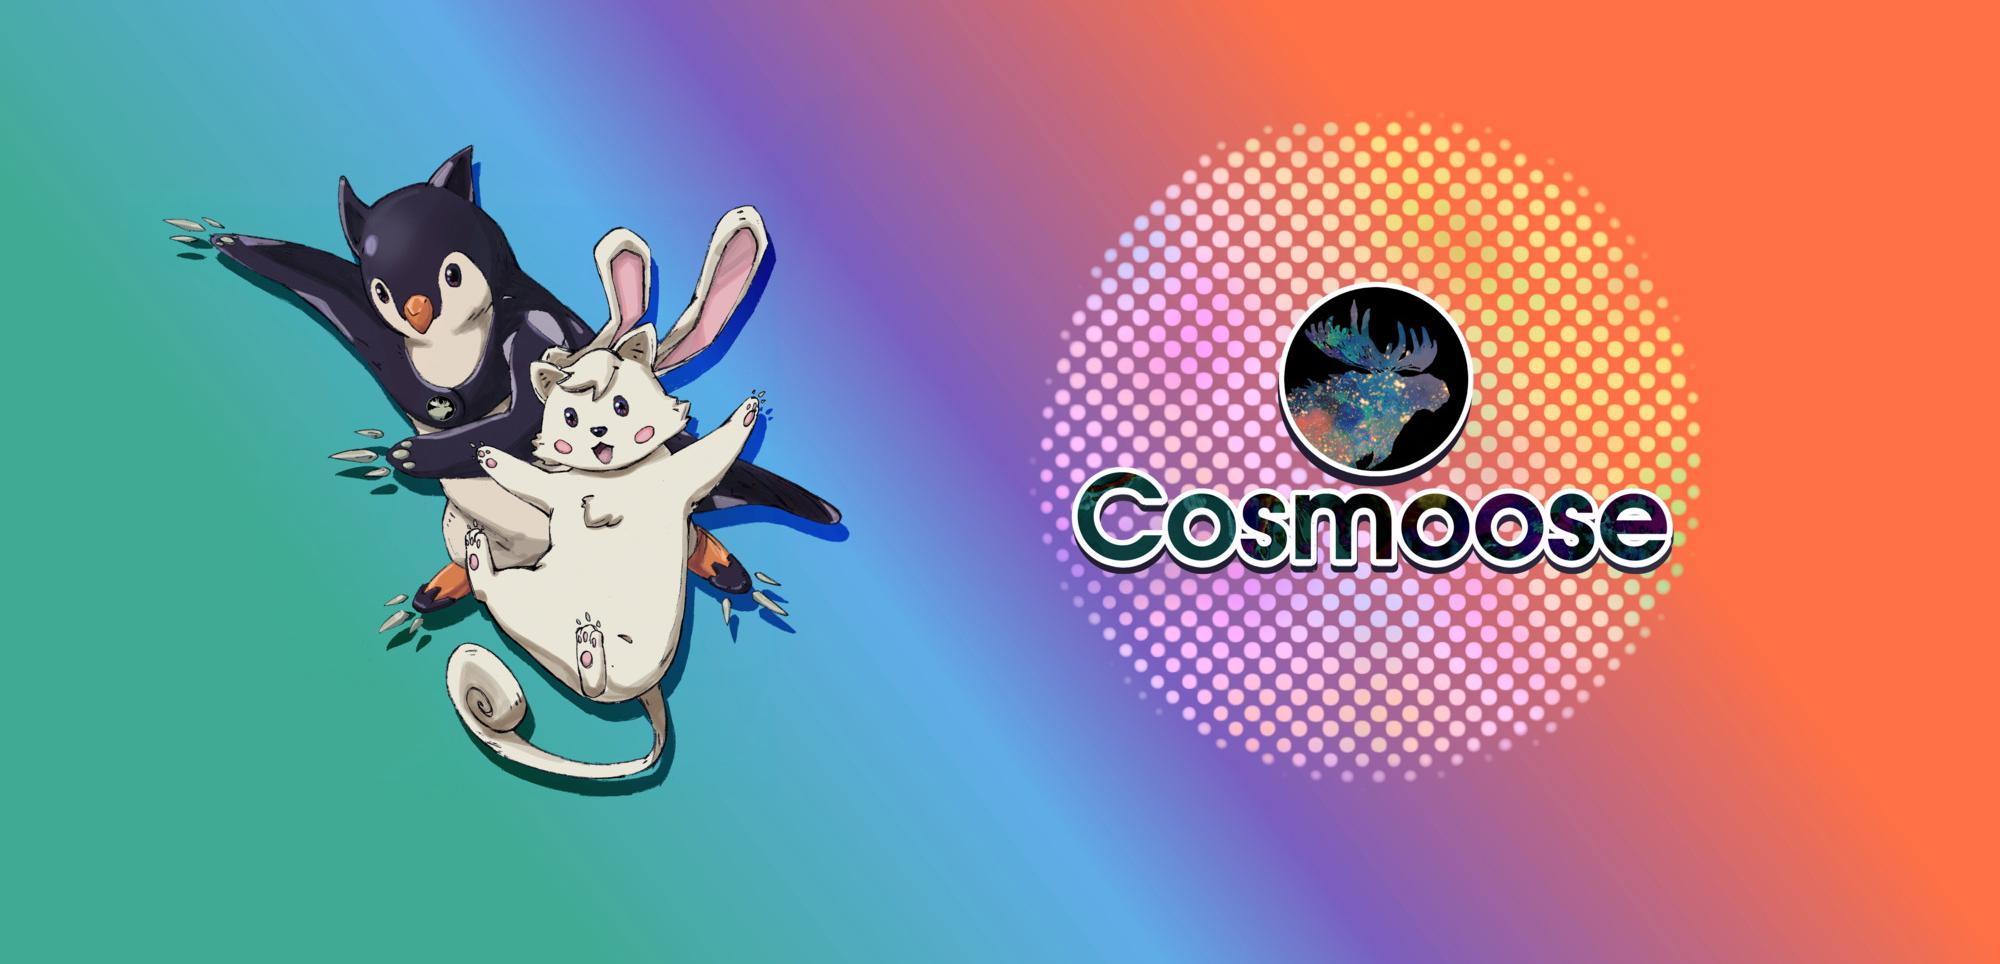
\includegraphics[height=.3\paperheight]{img/ccend}
\end{center}


\clearpage


\end{document}

